%!TEX program = xelatex
\documentclass[cn,hazy,blue,12pt,normal, math=newtx]{elegantnote}
\title{2021 年期末试题解析 }
\usepackage{newclude}
\author{}
\institute{彭康学导团}

\version{}
\date{}
\usepackage{pifont}
\usepackage{mathrsfs}
\usepackage{color}

\usepackage{array}

\begin{document}

\maketitle

\newpage
\section{选择题}
\include*{Part 1/1.1}
\include*{Part 1/1.2}
\include*{Part 1/1.3}
\include*{Part 1/1.4}
\include*{Part 1/1.5}
\section{填空题}
\include*{Part 2/2.1}
\include*{Part 2/2.2}
\include*{Part 2/2.3}
\include*{Part 2/2.4}
\include*{Part 2/2.5}
\section{计算题}
\include*{Part 3/3.1}
\include*{Part 3/3.2}
\paragraph*{3.3} 因为 $f'(x)=1-\dfrac{2}{1+x^2}$, 解得驻点为 $x=\pm 1$. 又 $f''(x)=\dfrac{4x}{\left(1+x^2\right)^2}$, 拐点为 $x=0$.

故
\begin{center}
\begin{tabular}{c|c|c|c|c|c|c|c}
\hline
$x$   & $(-\infty,-1)$ & $-1$ & $(-1,0)$       & $0$ & $(0,1)$         & $1$ & $(1,+\infty)$ \\ \hline
$f'$  & $+$            & $0$  & $-$            & $-$ & $-$             & $0$ & $+$           \\ \hline
$f''$ & $-$            & $-$  & $-$            & $0$ & $+$             & $+$ & $+$           \\ \hline
$f$   & $\uparrow$ 下凹  & 极大   & $\downarrow$ 下凹 & 拐点  & $\downarrow$ 上凹 & 极小  & $\uparrow$ 上凹 \\ \hline
\end{tabular}
\end{center}

$f$ 的单增区间为 $(-\infty,-1)\cup(1,+\infty)$, 单减区间为 $(-1,1)$.
\[
	f_{\max}=f(-1)=\dfrac{\pi}{2}-1,f_{\min}=f(1)=1-\dfrac{\pi}{2}
\]

$f$ 的图像在 $(-\infty,0)$ 下凹, 在 $(0,+\infty)$ 上凹, $(0,0)$ 是拐点.

渐近线: $x\to+\infty$ 方向为 $y=x-\pi$, $x\to-\infty$ 方向为 $y=x+\pi$. 

\begin{figure}[h]
	\centering
		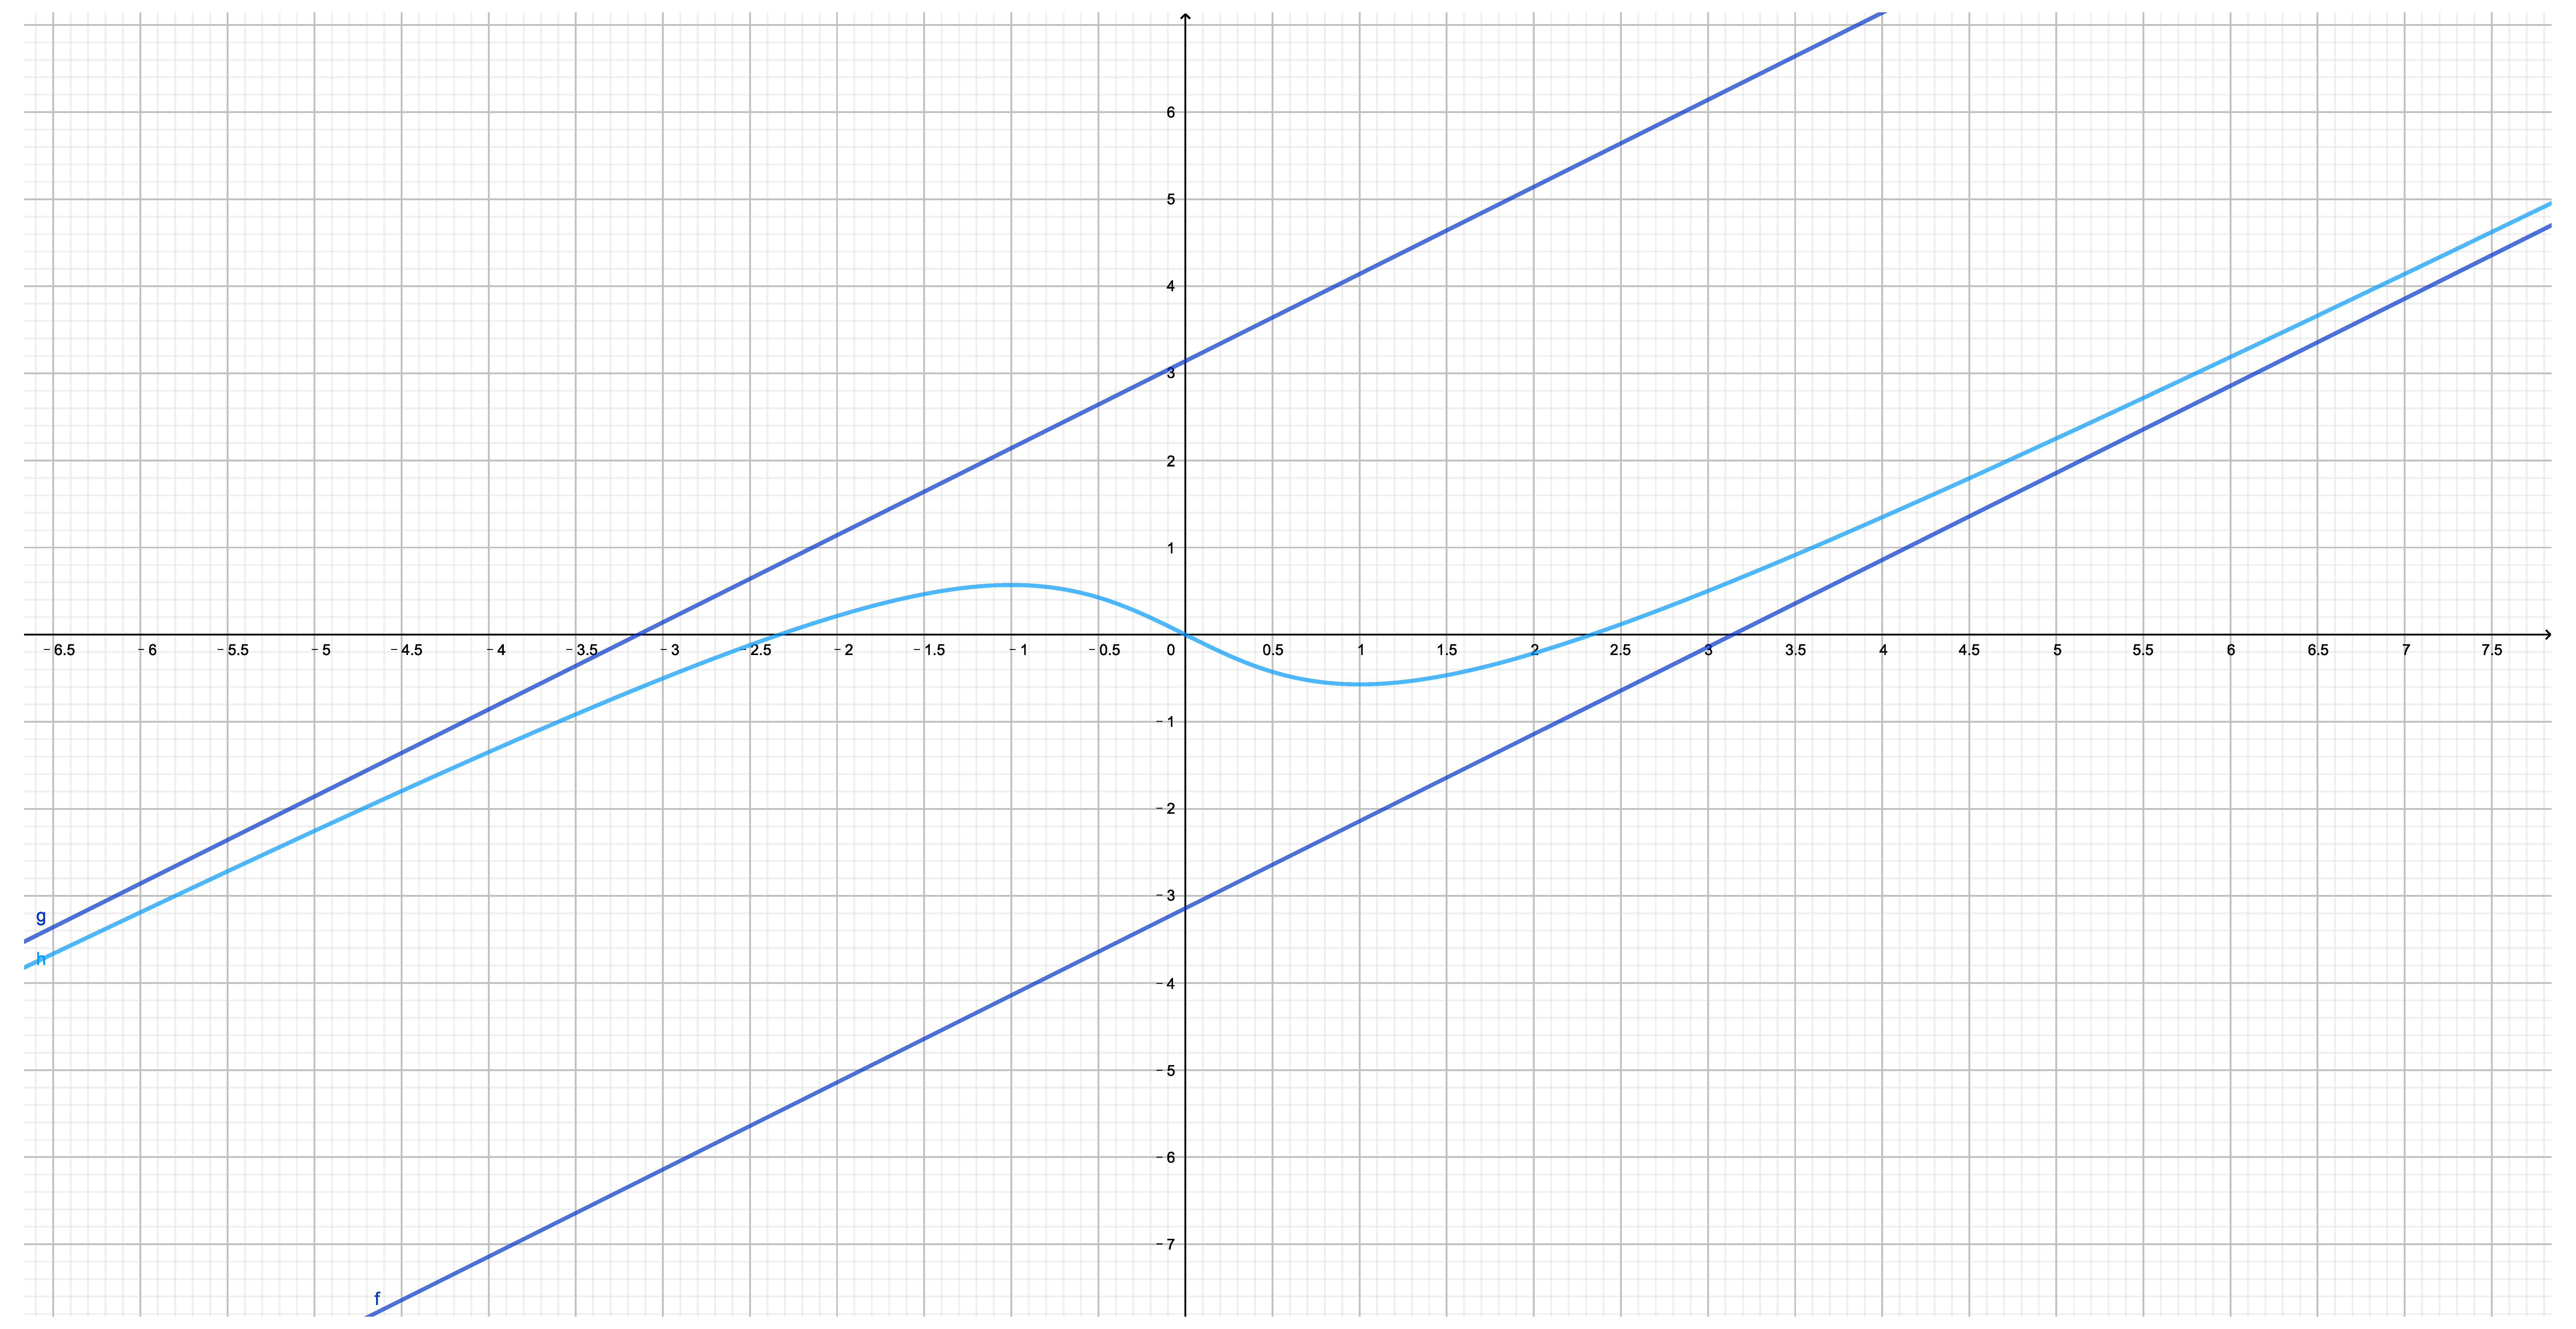
\includegraphics[scale = 0.1]{figure_3.3.pdf}
\end{figure}
\include*{Part 3/3.4}
\include*{Part 3/3.5}
\include*{Part 3/3.6}
\include*{Part 3/3.7}

\section{}

令
 $t=\ln (2 x-1)$, 则  $$\frac{\mathrm{d} t}{\mathrm{~d} x}=\frac{2}{2 x-1} \cdot$$ 
 
$$ \frac{\mathrm{d} y}{\mathrm{~d} x}=\frac{\mathrm{d} y}{\mathrm{~d} t} \frac{\mathrm{d} t}{\mathrm{~d} x}=\frac{2}{2 x-1} \frac{\mathrm{d} y}{\mathrm{~d} t}   \frac{\mathrm{d}^{2} y}{\mathrm{~d} x^{2}}=-\frac{4}{(2 x-1)^{2}} \frac{\mathrm{d} y}{\mathrm{~d} t}+\frac{4}{(2 x-1)^{2}} \frac{\mathrm{d}^{2} y}{\mathrm{~d} t^{2}}$$  代入原式, 化简得

$$ \frac{\mathrm{d}^{2} y}{\mathrm{~d} t^{2}}+\frac{\mathrm{d} y}{\mathrm{~d} t}-2 y=\frac{\mathrm{e}^{t}}{2}-\frac{1}{4}$$ 因此$$\lambda^{2}+\lambda-2=0\qquad \Longrightarrow\qquad\lambda_{1}=-2, \lambda_{2}=1 .$$ 齐次通解: $$ \tilde{y}=c_{1} \mathrm{e}^{-2 t}+c_{2}$$ 

$$\mathrm{e}^{t}   \frac{\mathrm{d}^{2} y}{\mathrm{~d} t^{2}}+\frac{\mathrm{d} y}{\mathrm{~d} t}-2 y=\frac{\mathrm{e}^{t}}{2} ,$$设特解为  $y_{1}^{*}=A t \mathrm{e}^{t}$ , 解得  $$y_{1}^{*}=\frac{t}{6} \mathrm{e}^{t}   \frac{\mathrm{d}^{2} y}{\mathrm{~d} t^{2}}+\frac{\mathrm{d} y}{\mathrm{~d} t}-2 y=-\frac{1}{4} ,$$ 易见特解为  $$y_{2}^{*}=\frac{1}{8} $$
通解为  $$y=c_{1} \mathrm{e}^{-2 t}+c_{2} \mathrm{e}^{t}+\frac{t}{6} \mathrm{e}^{t}+\frac{1}{8}=\frac{c_{1}}{(2 x-1)^{2}}+c_{2}(2 x-1)+\frac{2 x-1}{6} \ln (2 x-1)+\frac{1}{8} $$


\section{}
\textcolor{red}{解法一:}
  $|A-\lambda I|=\left|\begin{array}{ccc}2-\lambda & 1 & 0 \\ 0 & 2-\lambda & 0 \\ 0 & 1 & 3-\lambda\end{array}\right|=(\lambda-2)^{2}(3-\lambda)$ 
$\quad \therefore \lambda_{1}=\lambda_{2}=\mathbf{2}, \lambda_{3}=\mathbf{3}$  

对  $\lambda_{1}=\lambda_{2}=2,(A-2 I)^{2}=\left(\begin{array}{lll}0 & 0 & 0 \\ 0 & 0 & 0 \\ 0 & 1 & 1\end{array}\right) ,$ 解 $ (A-2 I)^{2} x=0$ , 得:  $$\vec{r}_{0}^{(1)}=\left(\begin{array}{l}1 \\ 0 \\ 0\end{array}\right)\qquad \vec{r}_{0}^{(2)}=\left(\begin{array}{l}0 \\ -1 \\ 1\end{array}\right)$$   
$$\vec{r}_{1}^{(1)}=(A-2 I) \vec{r}_{0}^{(1)}=0, \quad \vec{r}_{1}^{(2)}=(A-2 I) \vec{r}_{0}^{(2)}=(-1,0,0)^{T}$$   $$\vec{x}_{1}(t)=\mathrm{e}^{2 t}\left(\begin{array}{l}1 \\ 0 \\ 0\end{array}\right) \quad \vec{x}_{2}(t)=\mathrm{e}^{2 t}\left(\vec{r}_{0}^{(2)}+t \vec{r}_{1}^{(2)}\right)=\mathrm{e}^{2 t}\left(\begin{array}{c}-t \\ -1 \\ 1\end{array}\right)$$  

对  $\lambda_{3}=3 $, 解得特征向量为:  $\vec{r}_{3}=(0,0,1)^{T}$ . $\quad \vec{x}_{3}(t)=\mathrm{e}^{3 t}\left(\begin{array}{l}0 \\ 0 \\ 1\end{array}\right) $




齐次方程的基解矩阵为  $X_{1}(t)=\left(\vec{x}_{1}(t),-\vec{x}_{2}(t), \vec{x}_{3}(t)\right)=\left(\begin{array}{ccc}\mathrm{e}^{2 t} & t \mathrm{e}^{2 t} & 0 \\ 0 & \mathrm{e}^{2 t} & 0 \\ 0 & -\mathrm{e}^{2 t} & \mathrm{e}^{3 t}\end{array}\right)$ 

$$ \begin{aligned}
X(t) =X_{1}(t) X_{1}^{-1}(0) & =  \left(\begin{array}{ccc}
\mathrm{e}^{2 t} & \mathrm{e}^{2 t} & 0 \\
0 & \mathrm{e}^{2 t} & 0 \\
0 & -\mathrm{e}^{2 t} & \mathrm{e}^{3 t}
\end{array}\right)\left(\begin{array}{ccc}
1 & 0 & 0 \\
0 & 1 & 0 \\
0 & -1 & 1
\end{array}\right)^{-1} \\ & =\left(\begin{array}{ccc}
\mathrm{e}^{2 t} & t \mathrm{e}^{2 t} & 0 \\
0 & \mathrm{e}^{2 t} & 0 \\
0 & -\mathrm{e}^{2 t} & \mathrm{e}^{3 t}
\end{array}\right)\left(\begin{array}{lll}
1 & 0 & 0 \\
0 & 1 & 0 \\
0 & 1 & 1
\end{array}\right)=\left(\begin{array}{lcc}
\mathrm{e}^{2 t} & t \mathrm{e}^{2 t} & 0 \\
0 & \mathrm{e}^{2 t} & 0 \\
0 & \mathrm{e}^{3 t}-\mathrm{e}^{2 t} & \mathrm{e}^{3 t}
\end{array}\right) \end{aligned}$$

$$
X(t-\tau) \vec{f}(\tau)=X(t-\tau)\left(\begin{array}{l}
\tau \\
1 \\
0
\end{array}\right)=\left(\begin{array}{ccc}
\mathrm{e}^{2(t-\tau)} & (t-\tau) \mathrm{e}^{2(t-\tau)} & 0 \\
0 & \mathrm{e}^{2(t-\tau)} & 0 \\
0 & \mathrm{e}^{3(t-\tau)}-\mathrm{e}^{2(t-\tau)} & \mathrm{e}^{3(t-\tau)}
\end{array}\right)\left(\begin{array}{l}
\tau \\
1 \\
0
\end{array}\right)=\left(\begin{array}{c}
t \mathrm{e}^{2(t-\tau)} \\
\mathrm{e}^{2(t-\tau)} \\
\mathrm{e}^{3(t-\tau)}-\mathrm{e}^{2(t-\tau)}
\end{array}\right) \\
 $$

 
$$\int_{0}^{t} X(t-\tau) \vec{f}(\tau) \mathrm{d} \tau=\left(\begin{array}{c}
\frac{t}{2} \mathrm{e}^{2 t}-\frac{t}{2} \\
\frac{1}{2} \mathrm{e}^{2 t}-\frac{1}{2} \\
-\frac{1}{2} \mathrm{e}^{2 t}+\frac{1}{3} \mathrm{e}^{3 t}+\frac{1}{6}
\end{array}\right) \\$$

$$\text { 方程组通解为 } \\$$
$$\qquad \vec{x}=X(t) \vec{C}+\int_{0}^{t} X(t-\tau) \vec{f}(\tau) \mathrm{d} \tau=\left(\begin{array}{ccc}
\mathrm{e}^{2 t} & t \mathrm{e}^{2 t} & 0 \\
0 & \mathrm{e}^{2 t} & 0 \\
0 & \mathrm{e}^{3 t}-\mathrm{e}^{2 t} & \mathrm{e}^{3 t}
\end{array}\right)\left(\begin{array}{l}
C_{1} \\
C_{2} \\
C_{3}
\end{array}\right)+\left(\begin{array}{l}
\frac{t}{2} \mathrm{e}^{2 t}-\frac{t}{2} \\
\frac{1}{2} \mathrm{e}^{2 t}-\frac{1}{2} \\
-\frac{1}{2} \mathrm{e}^{2 t}+\frac{1}{3} \mathrm{e}^{3 t}+\frac{1}{6}
\end{array}\right) \\$$
$$=\left(\begin{array}{c}
C_{1} \mathrm{e}^{2 t}+\left(C_{2}+\frac{1}{2}\right) t \mathrm{e}^{2 t}-\frac{t}{2} \\
\left(C_{2}+\frac{1}{2}\right) \mathrm{e}^{2 t}-\frac{1}{2} \\
\left(C_{2}+C_{3}+\frac{1}{3}\right) \mathrm{e}^{3 t}-\left(C_{2}+\frac{1}{2}\right) \mathrm{e}^{2 t}+\frac{1}{6}
\end{array}\right) \quad \text { 其中 } \vec{C}=\left(\begin{array}{c}
C_{1} \\
C_{2} \\
C_{3}
\end{array}\right) \text { 任意. }$$
 

\textcolor{red}{解法二:}
$$\left\{\begin{array}{llrl}
\dot{x}_{1}=2 x_{1}+x_{2} & +t & & \cdots(1)  \\
\dot{x}_{2}= & 2 x_{2} & +1  & \cdots(2) \\
\dot{x}_{3}= & x_{2}+3 x_{3} &  & \cdots(3)
\end{array} \right.$$
其中(2)式的解为 $$x_{2}=\mathrm{e}^{\int 2 \mathrm{dt}}\left[\int \mathrm{e}^{-\int 2 \mathrm{dt}} \mathrm{d} t+C_{2}\right]$$
代入(1), 得:  $$\dot{x}_{1}-2 x_{1}=C_{2} \mathrm{e}^{2 t}-\frac{1}{2}+t, x_{1}=\mathrm{e}^{2 t}\left[\int\left(C_{2} \mathrm{e}^{2 t}-\frac{1}{2}+t\right) \mathrm{e}^{-2 t} \mathrm{~d} t+C_{1}\right]=C_{1} \mathrm{e}^{2 t}+C_{2} t \mathrm{e}^{2 t}-\frac{t}{2} $$
代入(3), 得:  $$\dot{x}_{3}-3 x_{3}=C_{2} \mathrm{e}^{2 t}-\frac{1}{2}, x_{3}=\mathrm{e}^{3 t}\left[\int\left(C_{2} \mathrm{e}^{2 t}-\frac{1}{2}\right) \mathrm{e}^{-3 t} \mathrm{~d} t+C_{3}\right]=-C_{2} \mathrm{e}^{2 t}+C_{3} \mathrm{e}^{3 t}+\frac{1}{6} $$
故方程组通解为  $$\vec{x}=C_{1} \mathrm{e}^{2 t}\left(\begin{array}{l}1 \\ 0 \\ 0\end{array}\right)+C_{2} \mathrm{e}^{2 t}\left(\begin{array}{l}t \\ 1 \\ -1\end{array}\right)+C_{3} \mathrm{e}^{3 t}\left(\begin{array}{l}0 \\ 0 \\ 1\end{array}\right)+\left(\begin{array}{c}-t / 2 \\ -1 / 2 \\ 1 / 6\end{array}\right) $$


$$=\left(\begin{array}{ccc}
\mathrm{e}^{2 t} & t \mathrm{e}^{2 t} & 0 \\
0 & \mathrm{e}^{2 t} & 0 \\
0 & -\mathrm{e}^{2 t} & \mathrm{e}^{3 t}
\end{array}\right)\left(\begin{array}{l}
C_{1} \\
C_{2} \\
C_{3}
\end{array}\right)+\left(\begin{array}{r}
-t / 2 \\
-1 / 2 \\
1 / 6
\end{array}\right)$$



\section{}
% \noindent\textcolor{red}{解:}
 
\noindent
\begin{enumerate}[(1)]
  \item 构造函数$F(x)=e^{\sin(x)}\mathscr{F}(x)$
$$\begin{aligned}
 F^{'}(x) &=\cos(x)e^{\sin(x)}\mathscr{F}(x)+e^{\sin(x)}\mathscr{F}^{'}(x)=(\cos(x)\mathscr{F}(x)+\mathscr{F}^{'}(x))e^{\sin(x)}
\end{aligned}$$

$\mathscr{F}(x)$在$(0,2\pi)$可导,$e^{\sin(x)}$在$(0,2\pi)$可导,
故$F(x)$在$(0,2\pi)$可导,$\mathscr{F}(x)$在$[0,2\pi]$连续,$F(x)$在$[0,2\pi]$连续
\item $F(0)=1$,$F(\pi)=3$,$F(2\pi)=2$,
又由于 $F(x)$连续,因此必有$a,b$满足$0<a<\pi<b<2\pi$
使得$$ F(a)=F(b)$$
且$F(x)$在$[a,b]$上连续,在$(a,b)$上可导,
故由罗尔定理知,
\(\exists\; \xi \in (a, b)\)使得$$F^{'}{(\xi)}=0$$

即$$e^{\sin(\xi)}(\mathscr{F}^{'}(\xi)+\mathscr{F}(\xi)\cos(\xi))=0$$

而$e^{\sin(\xi)}\ne 0$故在$(0,2\pi)$上至少有一点$\xi$,$\mathscr{F}^{'}(\xi)+\mathscr{F}(\xi)\cos(\xi)=0$

\end{enumerate}

  % \noindent
% \ding{173}



\section{}
% \textcolor{red}{解:}
$\left(1\right)$由题干条件$f(-x)+f(x)=A$,考虑代换$t=-x$,有
$$
\begin{aligned}
\int_{-a}^{a} f(x) g(x) d x & \stackrel{t=-x}{=}-\int_{a}^{-a} f(-t) g(-t) d t \\
& =\int_{-a}^{a} f(-t) g(t) d t, \\
\text{则} \int_{-a}^{a} f(x) g(x) d x & =\frac{1}{2}\left[\int_{-a}^{a} f(x) g(x) d x+\int_{-a}^{a} f(-x) g(x) d x\right] \\
& =\frac{1}{2} \int_{-a}^{a}[f(x)+f(-x)] g(x) d x \\
& =\frac{A}{2} \int_{-a}^{a} g(x) d x \stackrel{\left(\text{偶}\right)}{=} A \int_{0}^{a} g(x) d x .
\end{aligned}$$

$\left(2\right)$考虑到反正切函数特殊性,记 
$h(x)=\arctan(e^{x})$猜想$h(x)+h(-x)=C $ .
下面进行证明:$$\frac{\mathrm{d} }{\mathrm{d} x} {[h(x)+h(-x)]}=\frac{e^{x}}{1+e^{2x}} +\frac{-e^{-x}}{1+e^{-2x}}=0 $$

即$$h(x)+h(-x)=C=2h(0)=\frac{\pi}{2} $$

由(1)中结论有
$$
\begin{aligned}
&\int_{-\frac{\pi}{2} }^{\frac{\pi}{2}} \cos^4x\cdot \arctan(e^x)dx = \frac{\pi}{2} \int_{0}^{\frac{\pi}{2}} \cos^4x dx = \frac{\pi}{2} \times \frac{3}{4} \times \frac{1}{2} \times \frac{\pi}{2} = \frac{3 \pi^{2}}{32}
\end{aligned}
$$
注:华里士公式(Wallis)公式(书$P_{2.11} \text{例}3.21$)



$$\begin{aligned}
I_{n}&=\int_{0}^{\frac{\pi}{2}} \sin ^{n} x d x=\int_{0}^{\frac{\pi}{2}} \cos ^{n} x d x =\left\{\begin{aligned}
\displaystyle&\frac{(n - 1)!!}{n!!}, & &    n\text{为奇数} \\
\displaystyle& \frac{(n - 1)!!}{n!!}\cdot \frac{\pi}{2} , & &  n\text{为偶数}
\end{aligned}\right.
\end{aligned}$$




\end{document}
